% Based on free LaTex template https://www.overleaf.com/latex/templates/modelo-tcc-computacao-atitus/dgwsczcmpczz
\documentclass[14pt]{article}

\usepackage[a4paper, total={6in, 9in}]{geometry}

\usepackage[english, russian]{babel}
\usepackage{graphicx, url}
\usepackage[utf8x]{inputenc}
\usepackage[T1]{fontenc}
\usepackage[english=american]{csquotes}
\usepackage{float}
\usepackage{comment}
\usepackage{amsmath}
\usepackage{amssymb}
\usepackage{enumerate}
\usepackage{subcaption}
\usepackage{setspace}
\usepackage{listings}
\usepackage{inconsolata}
\usepackage{tabularray}

\usepackage[style=abnt]{biblatex}
\addbibresource{literature.bib}


\title{Colorizer}
\author{Бабанский Виталий, Бакин Денис}

\begin{document}

\maketitle

\section{Введение}

Задача восстановления цветных изображений из черно-белых снимков является распространенной задачи и применяется, например,
при обновлении исторических снимков, которые были сделаны до изобретения цветной фотографии.
Более сложной постановкой той же задачи считается раскрашивание снимков NIR (near-infrared spectroscopy) ---
это снимки, где вместо количества видимого света фотосенсором камеры подсчитывается количестве фотонов с длиной волны
от 780 нм до 2500 нм, то есть выше видимого диапазона. Такая съемка применяется при низкой освещенности и
при съемке архитектурных объектов.

\begin{figure}[H]
    \centering
    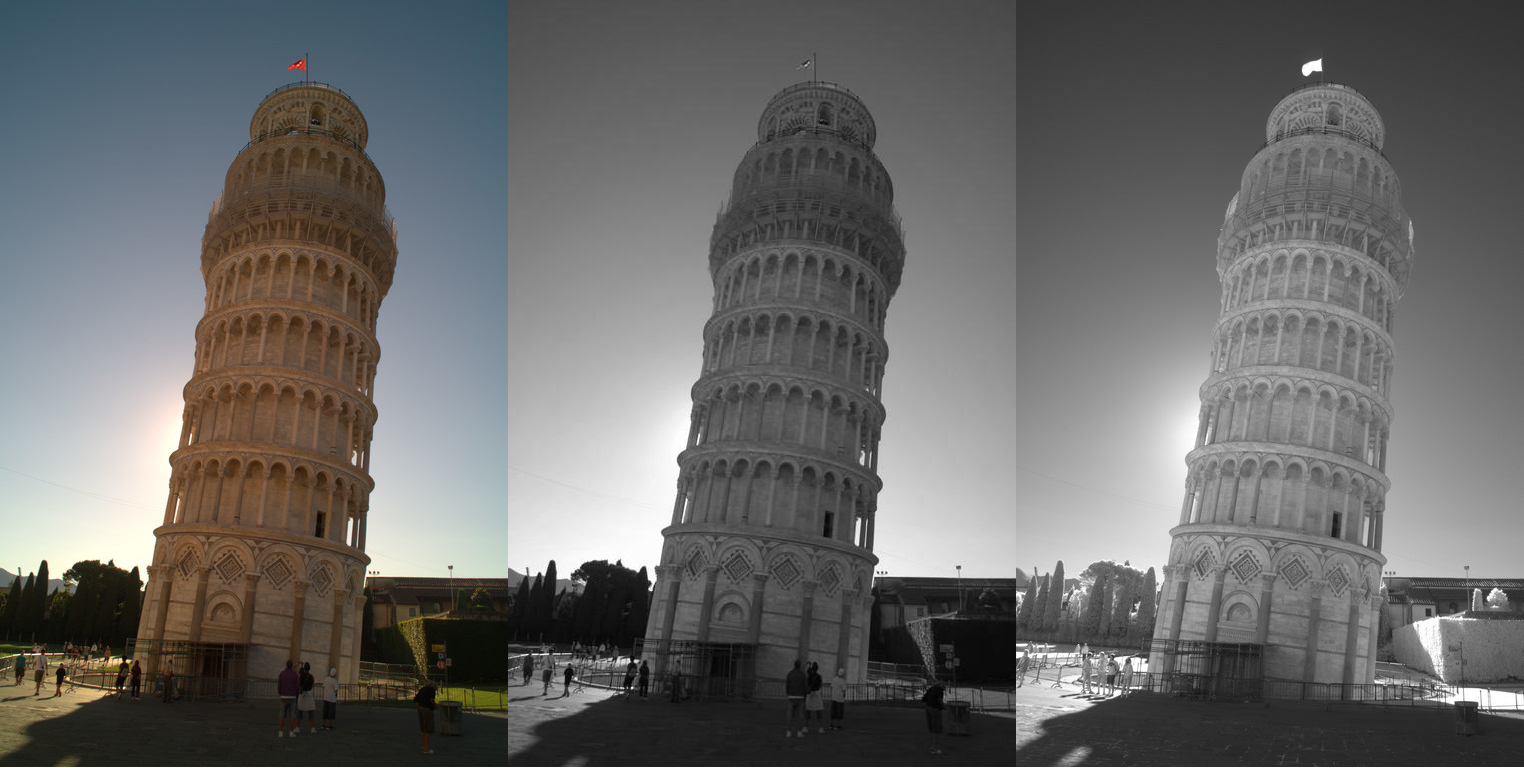
\includegraphics[width=0.5\textwidth]{resources/pisa_tower_3_colorspaces.jpg}
    \caption{Три пространства цветов: RGB, черно-белое и NIR}
    \label{fig:id_figura}
\end{figure}


\section{Постановка задачи}
Целью проекта является создание и обучение нейронной сети для получения цветных изображений по данным черно-белым изображениям,
а также провести ряд экспериментов, воспроизвести результаты выбранных статей и измерить полученное качество по набору метрик.


\section{Литература}
Список рассмотренных не окончательный. Включены только те статьи, идеи которых скорее всего будут использованы в реализации.

\subsection{Раскрашивание с подсказками}
\cite{GuidedImageColorization} предлагает архитектуру полносверточной нейронной сети, которая принимает на вход
черно-белое изображение и набор локальных и глобальных подсказок от пользователя. Сеть раскрашивает указанные пиксели так, как
скажет пользователь, а остальное изображение так, чтобы оно было наиболее естественным. Сеть показывает приемлемое качество
как бейзлайн: основная полносверточная нейросеть используется в некоторых других более сложных архитектурах. Отличная качество достигается
в особо сложных случаях, когда на снимке есть мелкий орнамент или цвета, которые сложно восстановить из контекста (воздушные шары, например).

\subsection{Instance colorization}
\cite{InstaColor} использует основную полносверточную нейронную сеть, из \cite{GuidedImageColorization}. Идея авторов заключается в генерации
ограничивающих прямоугольников (bounding boxes) вокруг известных объектов на изображении с помощью предтренированного детектора \cite{MaskCNN}.
Затем с помощью выбранного backbone раскрашиваются как вырезанные объекты, так и все изображение в целом. Затем на этапе карт признаков
модуль слияния "мягко" объединяет вырезанные раскрашенные объекты и полное раскрашенное изображение. Это дает улучшенные результаты по сравнению с прошлыми статьями
и относится к полностью автоматическому раскрашиванию черно-белых снимков.

\subsection{Cooperative colorization}
\cite{CoColor} авторы решают целых 2 проблемы: улучшают качество раскрашивания и предлагаются объединение и трансфер знаний модели между двумя доменами входных данных:
черно-белых и NIR изображений. В статье предлагается генерировать альтернативный домен по данному (NIR по черно-белому изображению или наоборот). Затем каждое
из изображений раскрашивается, результат объединяется. Поскольку такое количество генеративных сетей может отклоняться от ответа, авторы статьи предлагают множество дополнительных
ограничений для модели в виде функций потерь, которые требуют, чтобы раскрашенные изображения из разных доменов были очень похожи по структуре (ведь цвет ее не меняется).

\subsection{NIR-to-RGB Spectral Translation with Mamba}
\cite{ColorMamba} является лучшей на данный момент архитектурой для раскрашивания NIR изображений (на датасете NIR изображений с подготовленной валидационной выборкой
\cite{VCIP_2020_NIR_dataset}). Основа подхода заключается в построении двух наборов связанных модулей: сети для раскрашивания в пространство RGB,
сети для раскрашивания в пространство HSV, а также набора более компактных неглубоких подмодулей, описанных авторами статьи.

\begin{figure}[H]
    \centering
    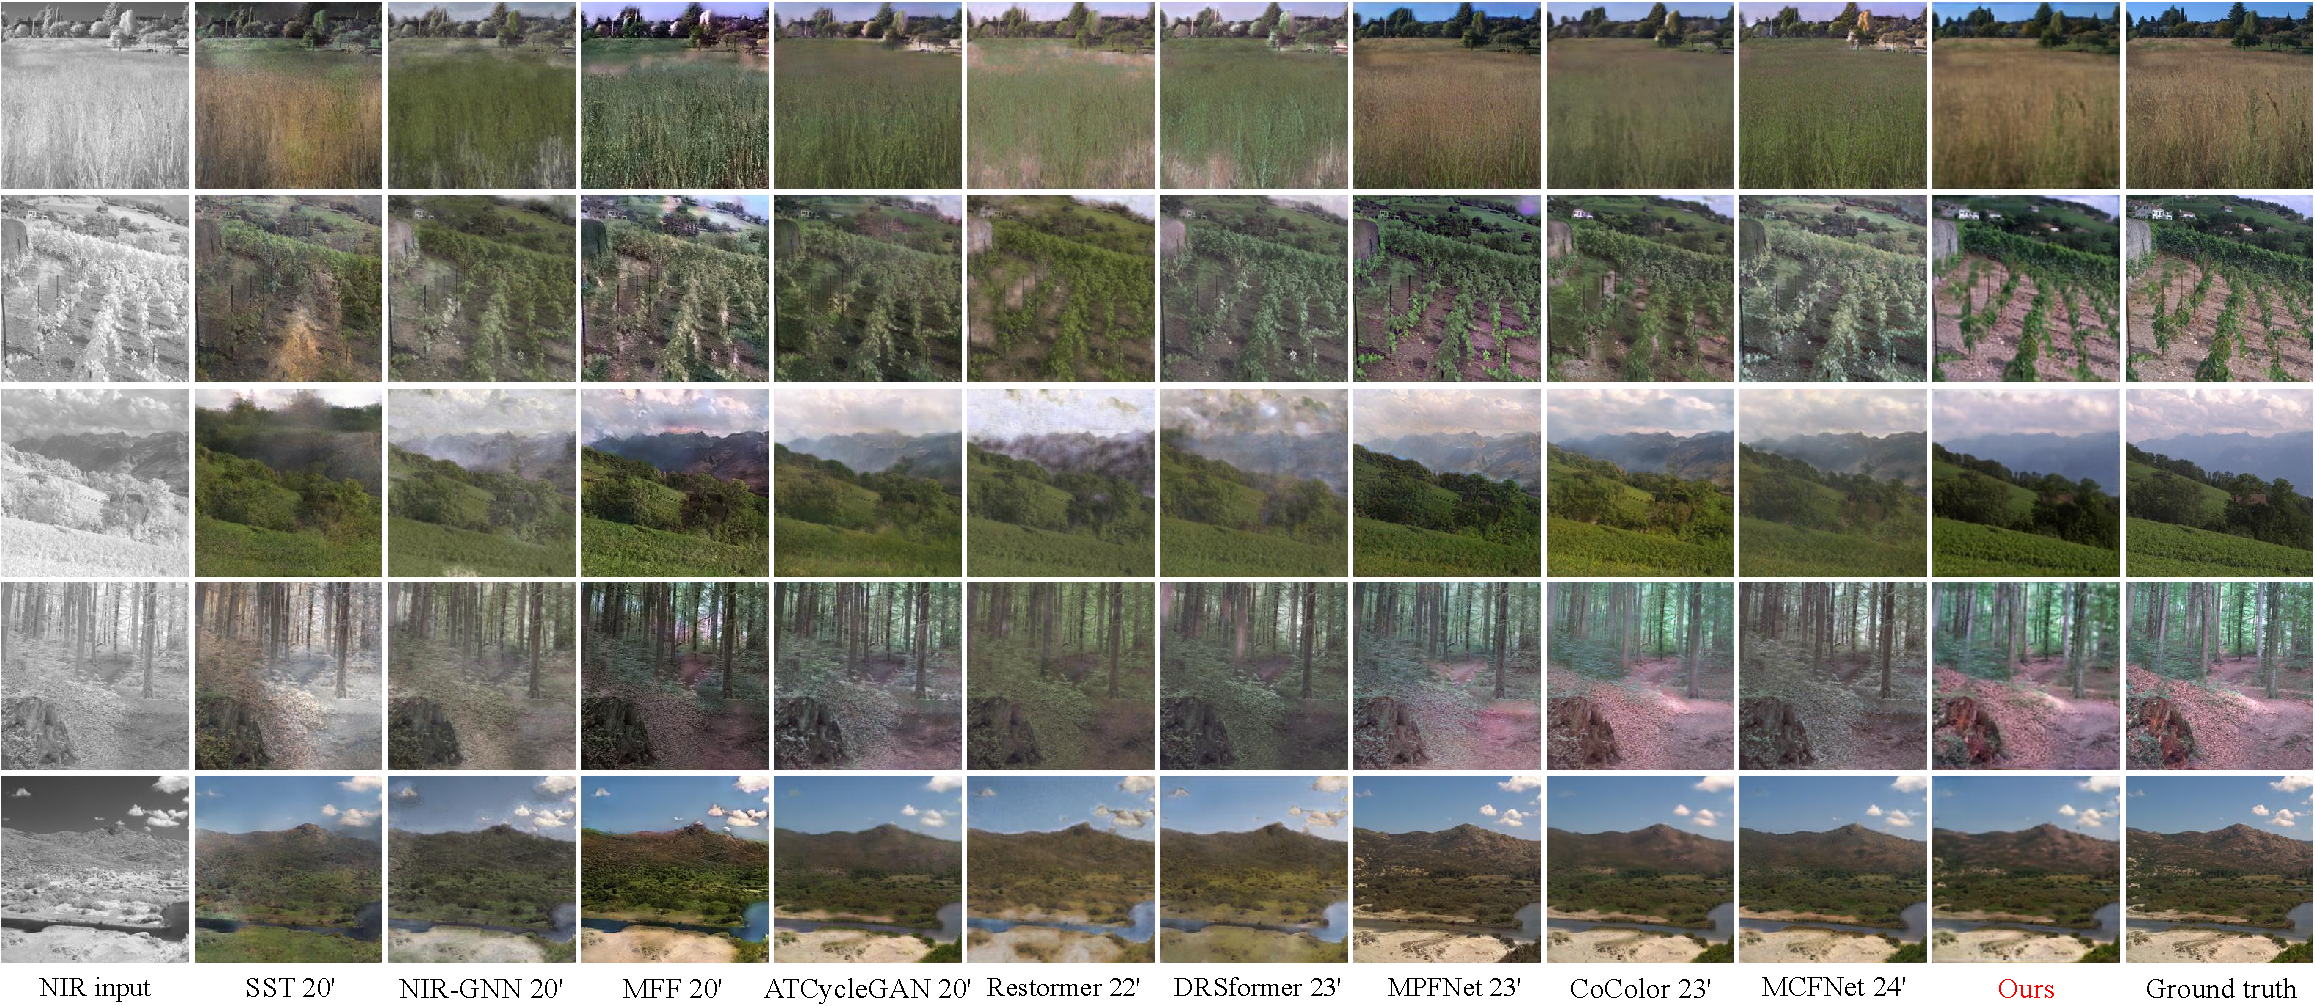
\includegraphics[width=1.05\textwidth]{resources/performance.pdf}
    \caption{Результаты работы ColorMambda \cite{ColorMamba}. Также приведено сравнение с CoColor \cite{CoColor}}
    \label{fig:id_figura}
\end{figure}


\section{Данные}
Авторы статей \cite{GuidedImageColorization}, \cite{InstaColor}, \cite{CoColor} использовали датасеты COCO \cite{COCO} и ImageNet \cite{ImageNet}.
Авторы статьи \cite{ColorMamba} использовали датасет NIR изображений с подготовленной валидационной выборкой \cite{VCIP_2020_NIR_dataset}.
Мы планируем использовать выборки из датасетов ImageNet, который содержит сфокусированные фотографии различных объектов, и COCO, который
содержит более общие сцены: архитектуры, природы.

Возможно, будут проведены эксперименты с созданием генерации черно-белого изображения по NIR данным. В этом случае к данным будет добавлен датасет
"RGB-NIR Scene Dataset".


\section{Метрики качества}
Для оценки качества раскрашивания снимков будем использовать набор метрик. По ним же будем сравнивать качество работы моделей.

\begin{itemize}
    \item \textbf{MSE}. Один из наиболее очевидных методов оценки близости предсказания к "верному" ответу.
    К недостаткам этой метрики можно отнести неразличимость мелкой зашумленности и отсутствия контроля за резкими переходами цветов,
    которые требуются при корректном раскрашивании изображений.
    $$
        MSE(I_1, I_2) = \sum_{x=1}^{W} \sum_{y=1}^{H} \frac{(I_1(x,y) - I_2(x,y))^2}{W \cdot H}
    $$

    \item \textbf{PSNR (Пиковое отношение сигнал/шум)}: PSNR измеряет качество цветных изображений, сравнивая пиксельные различия между оригиналом и
    раскрашенным изображением. Более высокие значения PSNR указывают на лучшее качество изображения с меньшими искажениями.
    $$
        PSNR(I_1, I_2) = 10 \cdot \log_{10} \left( \frac{MAX^2}{MSE(I_1, I_2)} \right)
    $$
    где $MAX$ --- максимальное значение пикселя (например, 255 для 8-битных изображений).

    \item \textbf{SSIM (Индекс структурного сходства)}: SSIM оценивает структурное сходство между оригиналом и раскрашенным изображением,
    учитывая яркость, контрастность и текстуру. Этот индекс предоставляет более точную для восприятия меру качества изображения по сравнению
    с метриками на основе пикселей, такими как PSNR.
    $$
        SSIM(I_1, I_2) = \frac{(2 \mu_1 \mu_2 + C_1)(2 \sigma_{12} + C_2)}{(\mu_1^2 + \mu_2^2 + C_1)(\sigma_1^2 + \sigma_2^2 + C_2)}
    $$
    где $\mu_1$ и $\mu_2$ --- средние значения яркости оригинала и раскрашенного изображения, $\sigma_1^2$ и $\sigma_2^2$ --- дисперсии,
    $\sigma_{12}$ --- ковариация, а $C_1$ и $C_2$ --- константы для стабилизации деления. По приведенной формуле метрика считается локально,
    а затем усредняется по всему изображению.


    \item \textbf{AE (Абсолютная ошибка)}: AE количественно оценивает абсолютное различие между соответствующими пикселями оригинала и
    раскрашенного изображения. Меньшие значения AE указывают на лучшую точность раскраски.
    $$
        AE(I_1, I_2) = \sum_{x=1}^{W} \sum_{y=1}^{H} \frac{|I_1(x,y) - I_2(x,y)|}{W \cdot H}
    $$


    \item \textbf{LPIPS (Обученное перцептуальное сходство изображений)} \cite{PerceptualMetric}: LPIPS оценивает перцептуальное сходство с использованием моделей
    глубокого обучения, фокусируясь на том, как человеческое зрение воспринимает различия между оригиналом и раскрашенным изображением.
    Более низкие значения LPIPS означают, что раскрашенным изображение более точно соответствует восприятию человека.
    $$
        LPIPS(I_1, I_2) = \frac{1}{N} \sum_{i=1}^{N} \| f_i(I_1) - f_i(I_2) \|_2^2
    $$
    где $f_i$ --- выходные данные $i$-го слоя предобученной модели, а $N$ --- количество слоев.
\end{itemize}


\section{Текущая идея}
Идея на момент написания отчета и вероятно изменится в будущем.

В качестве бейзлайна хочется реализовать полносверточную нейронную сеть из \cite{GuidedImageColorization} и провести ряд экспериментов, возможно,
с реализацией интерактивных подсказок в пользовательском интерфейсе. Затем хотелось бы реализовать одну из других рассмотренных статей и проверить
воспроизводимость результатов по выбранным метрикам.


\section{Бейзлайн}
В качестве бейзлайна согласно \cite{GuidedImageColorization} была выбрана полносверточная нейронная сеть --- UNet, которая изначально была
предложена для сегментации медицинских изображений, \cite{UNetForMedSegmentation}. На вход такая сеть получает одноканальное изображение
(более подробно преобразования изображений будут описаны в следующем разделе), затем применяет набор сверток с residual connections, сокращая
в текущей модицикации размер изображений в 8 раз по каждому измерению, после чего upscale свертками восстанавливает его исходные размер.

Выход сети --- двуканальное изображение, которое в изначальной статье интерпретировалось как распределение по двум классам каждого из пикселей:
наибольшая вероятность у того класса маски сегментации, к которому скорее всего приналежит текущий пиксель. В нашем бейзлайне двуканальный выход сети интерпретировался
как два нормированных цветовых канала.

\begin{figure}[H]
    \centering
    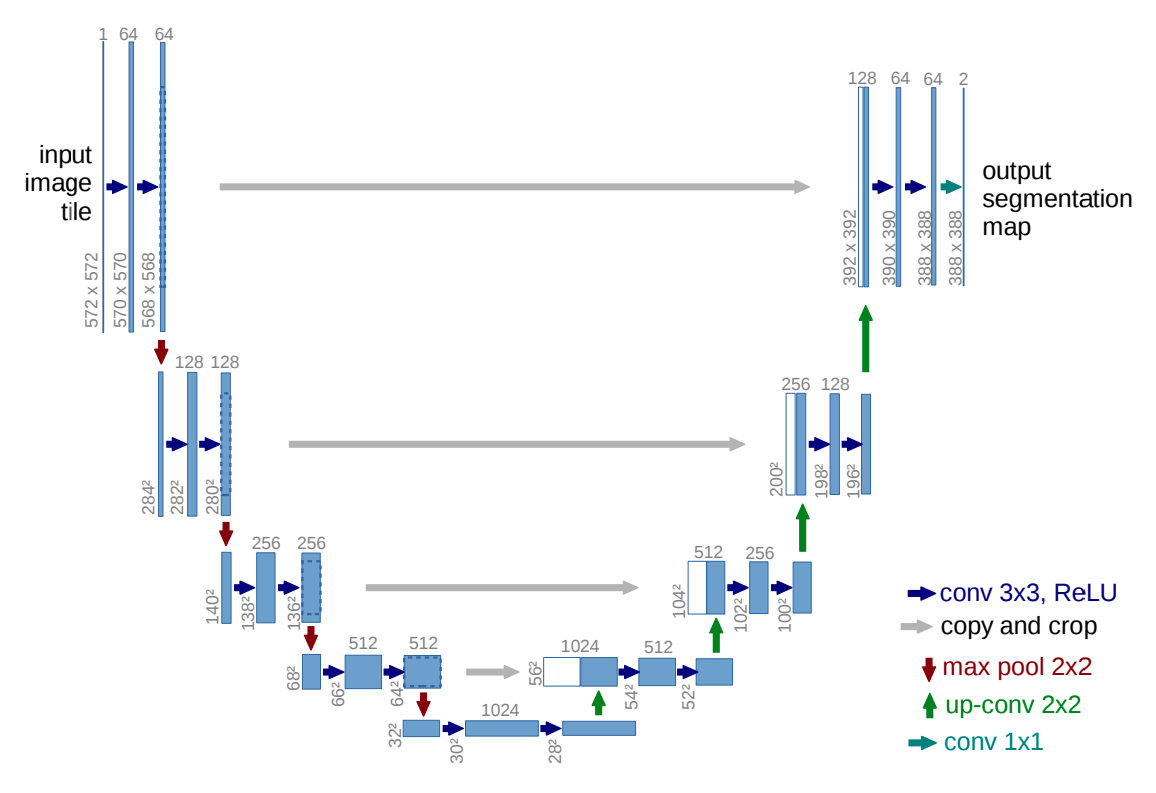
\includegraphics[width=0.5\textwidth]{resources/u_net_architecture.png}
    \caption{UNet архитекрута (пример для 32х32 в середине сети). Каждый голубой прямоугольник соответствует
    многоканальной карте признаков}
    \label{fig:id_figura}
\end{figure}

\section{Обучающий пайплайн}
Опишем, какие преобразование применяются к изображениям.
\begin{enumerate}
    \item Читаем RGB изображение
    \item Преобразуем RGB изображение в цветовое пространство CIELab и разделяем на одиночный канал $L$ -- яркость пикселей, вход сети и
        и на двуканальную матрицу $ab$
    \item нормируем $L$ и $ab$ на максимальные значение по каналам: $100$ и $255$ соответственно
    \item подаем $L$ на вход сети, получаем $ab$
    \item денормируем каналы
    \item совмещаем в трехкальное CIELab изображение и преобразуем обратно в RGB
    \item показываем пользователю или сохраняем
\end{enumerate}

Для удобства разработки и постановки экспериментов используется создание и сохранение логов с помощью библиоткеи Wandb,
в репозитории сохраняется модульная архитектура Python файлов, почти везде выбран объектно-ориентированный подход. Например,
в классе \texttt{Trainer} одноименного модуля реализована вся логика, связанная с обучением, дообучением, сохранением, загрузкой, тестированием моделей
с выбранной функцией потерь, оптимизатором и загрузчиком данных для обучения, валидации и тестирования.

Ссылка на репозиторий: \url{https://github.com/dfbakin/colorizer/tree/checkpoint-1-baseline}



\section{Путь к бейзлайну}
\subsection{Проблемы с функцией потерь}

Изначально предполагалось использовать UNet для раскрашивания изображений, но обучение такой модели
не дало приемлемых результатов. Предположительно из-за усреднения функции потерь по всем пикселям изображения
нейросеть находила оптимум при генерации усредненного цвета: оттенка серого или желтого. Это может происходить
из-за слишком малого вклада каждого из пикселей в итоговое значение функции потерь, а
обратное распространение ошибки оптимизирует все изображение в целом, а не каждый пиксель по отдельности.

\begin{figure}[H]
    \centering
    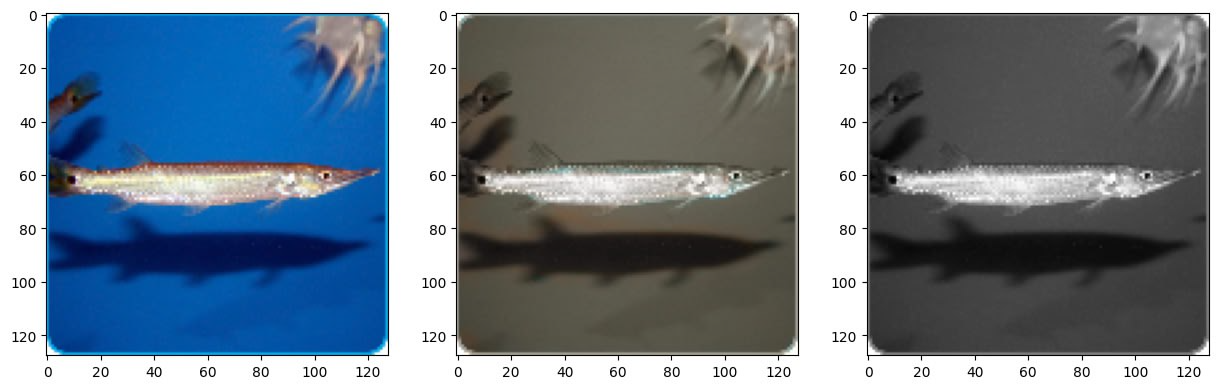
\includegraphics[width=1.0\textwidth]{resources/bad_fish_colorization.png}
    \caption{Слева направо: ground truth, раскрашенное UNet, L-канал преобразованного изображение}
    \label{fig:id_figura}
\end{figure}


\begin{figure}[H]
    \centering
    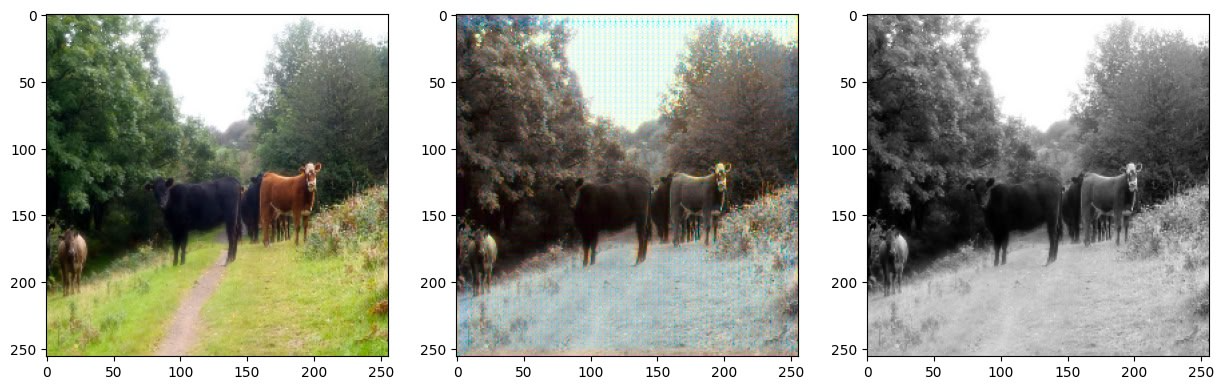
\includegraphics[width=1.0\textwidth]{resources/bad_cows_colorization.png}
    \caption{Слева направо: ground truth, раскрашенное UNet, L-канал преобразованного изображение}
    \label{fig:id_figura}
\end{figure}

В качестве фукнции потерь использовались как MSE, так и HuberLoss с подобранными гиперпараметрами, чтобы избежать влияния выбросов на функцию потерь. Это не дало
приемлемых результатов.

\subsection{Изменение подхода к обучению}

Чтобы раскрашивать изображение с вниманием к отдельных пикселей и малым областям разных цветов, парадигма обучения была изменена на генеративно-состязательную нейросеть (GAN).
В частности, генератором осталась UNet, а дискриминатором была выбрана сверточная нейросеть, которая за несколько блоков сверток
старается предсказать, является ли изображение изначально раскрашенным (истинным) либо сгенерированным. В качестве функции потерь для генератора может использоваться
BinaryCrossEnthropy (возможно, с изначальными применением сигмоидной функции активации, если на вход подаются логиты вместо вероятностей) или MSE. Функцией
потерь для генератора выступает L1Loss.

Обратное распространение и состязательность в обучении тогда сконструировна следующим образом (для каждого батча):
\begin{enumerate}
    \item Пропускаем истинное изображение через дискриминатор, считаем функцию потерь. Аналогично с сгенерированным изображением.
    Усредняем полученные значения функций потерь GAN-а и выполняем back propagation;
    \item Делаем шаг оптимизатора для дискриминатора;
    \item Замораживаем расчет и изменение градиентов дискриминатора, чтобы при оптимизации генератора веса сверточного дискриминатора не изменялись;
    \item Считаем функцию потерь заморженного генератора на сгенерированным изображении как если бы оно было истинным. По сути
    находим, насколько мы далеки от успешного "обмана" дискриминатора. Также считаем функцию потерь (L1Loss), чтобы оставлять одной из важных целей
    близость к истинному изображению, а не только "обман" дискриминатора.
    Складываем функции потерь с определенными заранее весами и выполняем back propagation;
    \item Делаем шаг оптимизатора для генератора;
    \item Размораживаем градиенты дискриминатора, можем переходить к следующем батчу.
\end{enumerate}

Генерация изображений во время инференса происходит с использованием генератора: обученная описанным образом UNet принимает на вход
$L$ канал изображения, а на выходе выдает два канала $ab$.

Такой подход стал давать более разнообразные цвета, сложнее учиться, но сходимость также не была достигнута

\begin{figure}[H]
    \centering
    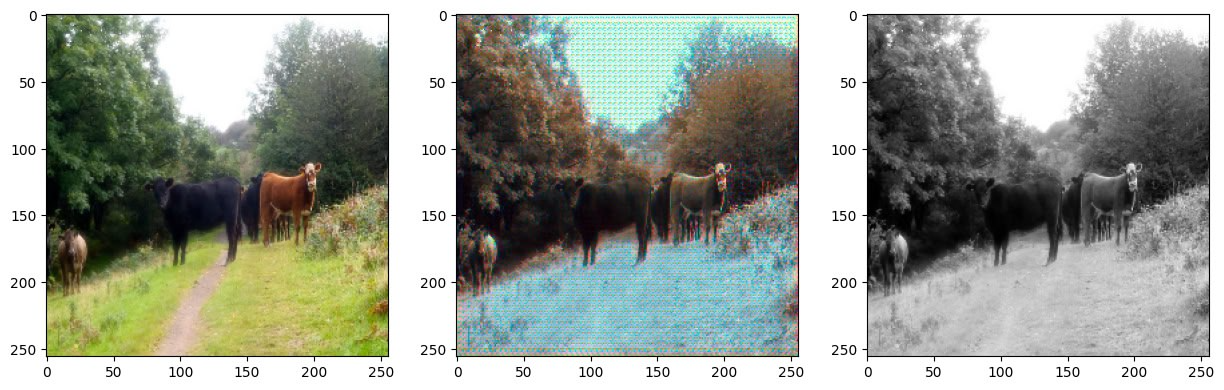
\includegraphics[width=1.0\textwidth]{resources/middle_of_gan_baseline.png}
    \caption{Результаты раннего обучения GAN бейзлайна. Слева направо: ground truth, раскрашенное UNet, черно-белое изображение. Стоит отметить,
    что области изображения (трава и животные) визуально выделены верно, но цвета не соответствуют действительности}
    \label{fig:id_figura}
\end{figure}

\subsection{Предобучения генератора}

Следующей идеей, которая привела к итоговому бейзлайну, стало предобучение генератора на
MSE функции потерь. В частности, чередование состязательного лосса и MSE дало приблизительно такой результат


\begin{figure}[H]
    \centering
    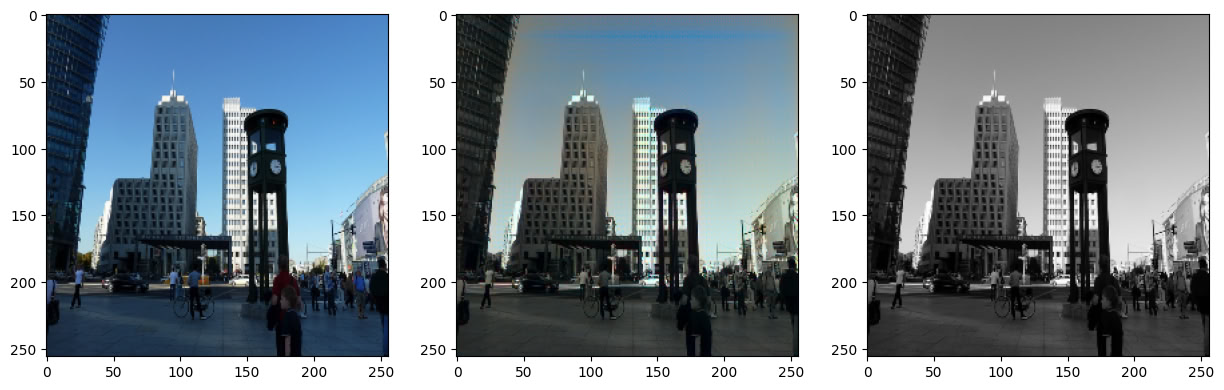
\includegraphics[width=1.0\textwidth]{resources/gan_and_chaos_pretrain.png}
    \caption{Cherry-picking. Только для демонстрации, что такой подход может на конкретном изображении хорошо показывать небо}
    \label{fig:id_figura}
\end{figure}


Идея предобучения генератора получила свое продолжение в виде использования весов ResNet18, полученных обучением
на ImageNet1000. Из одноканального изображения $L$ получаем трехканальное изображение через добавление первого сверточного слоя
с $\text{n\_filters}=3$, слои финального пуллинга и классификации были удалены.

Описанный backbone использовался как encoder в UNet. К слоям-сверток после функций активации добавлялись skip-коннекты, которые
необходимы для декодера UNet. Генеративно-состязательный подход к обучения остался прежним.

Классическая UNet была заменена на Dynamic UNet (\cite{yang2024dynamicunetadaptivelycalibrate}). Ниже приведены
первые результаты (5 эпох предобучения генератора, 1 эпоха обучения полного GAN. Все на половине датасета COCO Things test 2017).

\begin{figure}[H]
    \centering
    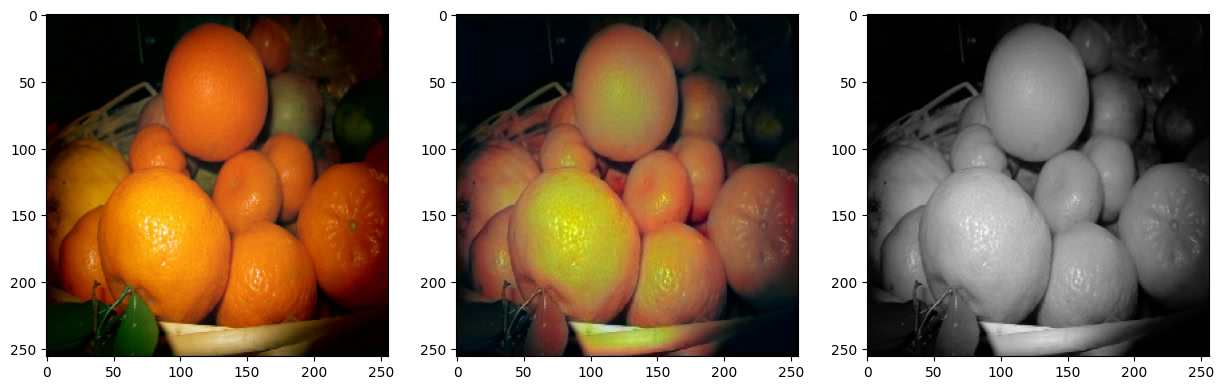
\includegraphics[width=1.0\textwidth]{resources/dynamic_unet_gan_results/oranges.png}
    \caption{Dynamic UNet GAN result: Oranges}
    \label{fig:oranges}
\end{figure}

\begin{figure}[H]
    \centering
    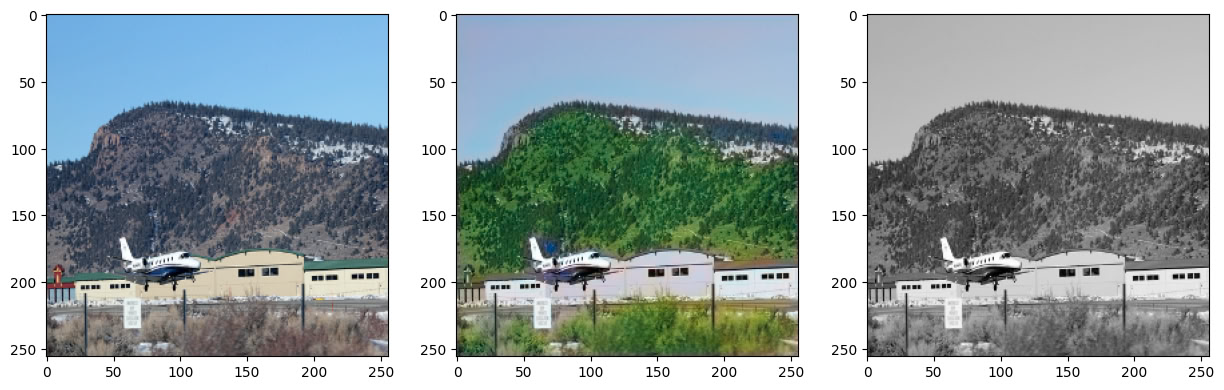
\includegraphics[width=1.0\textwidth]{resources/dynamic_unet_gan_results/plane_and_hill.png}
    \caption{Dynamic UNet GAN result: Plane and Hill}
    \label{fig:plane_hill}
\end{figure}

\begin{figure}[H]
    \centering
    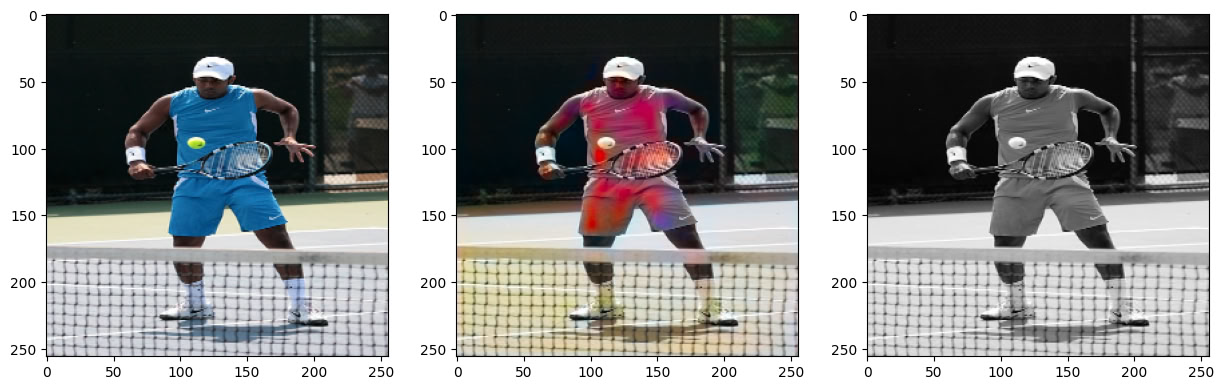
\includegraphics[width=1.0\textwidth]{resources/dynamic_unet_gan_results/tennis_player.png}
    \caption{Dynamic UNet GAN result: Tennis Player}
    \label{fig:tennis_player}
\end{figure}

\begin{figure}[H]
    \centering
    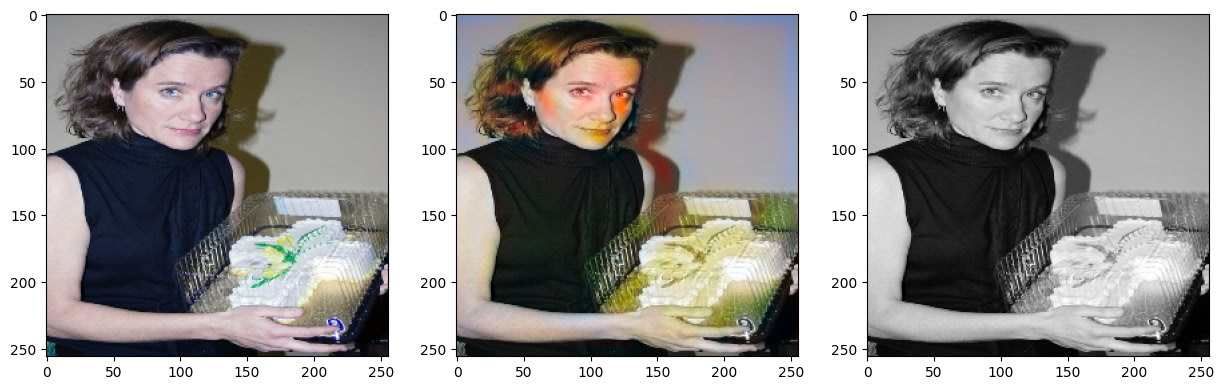
\includegraphics[width=1.0\textwidth]{resources/dynamic_unet_gan_results/woman.png}
    \caption{Dynamic UNet GAN result: Woman}
    \label{fig:woman}
\end{figure}

Стоит отметить, что некоторые цвета могут не соответствовать наблюдаемым в реальности,
но их расположение и сегментация по различным цветам передается весьма точно.

\subsection{Итог построения измененного бейзлайна}

В итоге за бейзлайн была выбрана генеративно-состязательная сеть, которая
использует в качестве генератора UNet с предобученным ResNet18 backbone.




\section{Подготовка эффективного инференса}

Чтобы подготовить эффективный инференс, необходимо оптимизировать модель, чтобы она требовала как можно меньшего количества
операций с плавающей точкой (FLOPS) и памяти. Для этого можно применить несколько методов:

\begin{itemize}
    \item \textbf{Quantization}: уменьшение точности весов и активаций модели, что позволяет снизить требования к памяти и ускорить вычисления.
    \item \textbf{Pruning}: удаление незначительных весов из модели, что позволяет уменьшить ее размер и ускорить инференс.
    \item \textbf{Knowledge Distillation}: обучение компактной модели (студента) на основе более крупной модели (учителя), что позволяет сохранить производительность при меньших затратах ресурсов.
\end{itemize}

\subsection{Дистилляция}

Дистилляция — это метод, позволяющий обучить компактную модель (студента) на основе более крупной модели (учителя).
В данном случае в качестве учителя используется модель
UNet с предобученным ResNet18 в качестве энкодера, а в качестве студента — уменьшенная версия UNet с меньшим числом фильтров и уровней декодера.

Для дистилляции используется комбинированная функция потерь, которая состоит из двух частей:
\begin{enumerate}
    \item \textbf{Soft Loss}: измеряет расхождение между распределениями вероятностей, предсказанными учителем и студентом. Для этого используется KL дивергенция.
    Идея заключается в том, что учительская модель обобщила больше информации за счет сложности своей архитектуры и если
    меньшая модель будет пытаться имитировать ее поведение, то она сможет лучше обобщать информацию.
    $$
    L_{\text{soft}} = \text{KLDiv} \left( \text{log\_softmax}\left(\frac{S}{T}\right), \text{softmax}\left(\frac{T}{T}\right) \right) \cdot \alpha \cdot t^2
    $$
    где $ S $ — предсказания студента, $ T $ — предсказания учителя, $ t $ — параметр температуры,
    который сглаживает распределение вероятностей, а $ \alpha $ — весовой коэффициент для мягкой потери.

    \item \textbf{Жесткая потеря (Hard Loss)}: измеряет расхождение между предсказаниями студента и истинными метками (ground truth). Для этого используется MSE (Mean Squared Error):
    $$
    L_{\text{hard}} = \text{MSE}(S, Y) \cdot (1 - \alpha)
    $$
    где $ Y $ — истинные метки (ground truth).
\end{enumerate}

Итоговая функция потерь:
$$
L_{\text{distillation}} = L_{\text{soft}} + L_{\text{hard}}
$$

\subsubsection*{Алгоритм дистилляции}
Для каждого батча данных:
\begin{enumerate}
    \item Учительская модель предсказывает выходные значения $ T $ (teacher output).
    \item Студенческая модель предсказывает выходные значения $ S $ (student output).
    \item Вычисляется комбинированная функция потерь $ L_{\text{distillation}} $.
    \item Выполняется обратное распространение ошибки (backpropagation) и обновление весов студенческой модели.
\end{enumerate}



\subsubsection*{Результаты}
Дистилляция позволяет значительно уменьшить размер модели и ускорить инференс,
сохраняя при этом приемлемое качество.
Итоговые метрики и время инференса приведены в таблице \ref{tab:lpips_inference_comparison}.


\subsection{Итоговые метрики и время инференса}


\begin{table}[H]
    \centering
    \begin{tabular}{|c|c|c|}
        \hline
        \textbf{Model} & \textbf{LPIPS Metric} & \textbf{Inference Time (ms)} \\ \hline
        Original Model & 0.011 & 150 \\ \hline
        Pruned Model & 0.012 & 150 \\ \hline
        Distilled Model & 0.0649 & 9 \\ \hline
    \end{tabular}
    \caption{Сравнение методов опмизации по LPIPS метрике и времени инференса}
    \label{tab:lpips_inference_comparison}
\end{table}


\pagebreak
\printbibliography

\end{document}
